\chapter{Research framework}
Majority of the most popular fluid surface reconstruction methods are using level set technique for construction of fluid surface mesh. Given fluid particle displacement , density and other SPH information this methods are computing scalar distance field (SDF) values for previously defined 3D grid domain. After computation of the SDF values this methods apply marching cubes algorithm to construct to determine surface surface vertices.
Thus  smoothing algorithms, described in this thesis are designed in the way that they can be applied on the reconstruction algorithms with described infrastructure.


In this thesis next methods were implemented for surface reconstruction:
\begin{itemize}
  \item \emph{Density based reconstruction} described in \cite{DencRec}. This method uses SPH particle density information to compute level set scalar field, with the domain of SDF values from $[initialValue, initialValue+1]$.
  \item \emph{Zhu-Bridson} method, described in \cite{ZhuBridson}, which uses SPH particle displacement for computing level set
  \item \emph{Solenthaler} method first introduced in \cite{Solenthaler}. This method exploits the idea of Zhu-Bridson technique, but improves the computation of level set to remove artifact of Zhu-Bridson method in concave areas.
\end{itemize}



\section{Framework architecture}
To simplify further framework development and testing spacial care was applied to design the class hierarchy. The class diagram is presented in the Figure \ref{fig:class-diagam}.

\begin{figure}[H]

	\begin{center}
	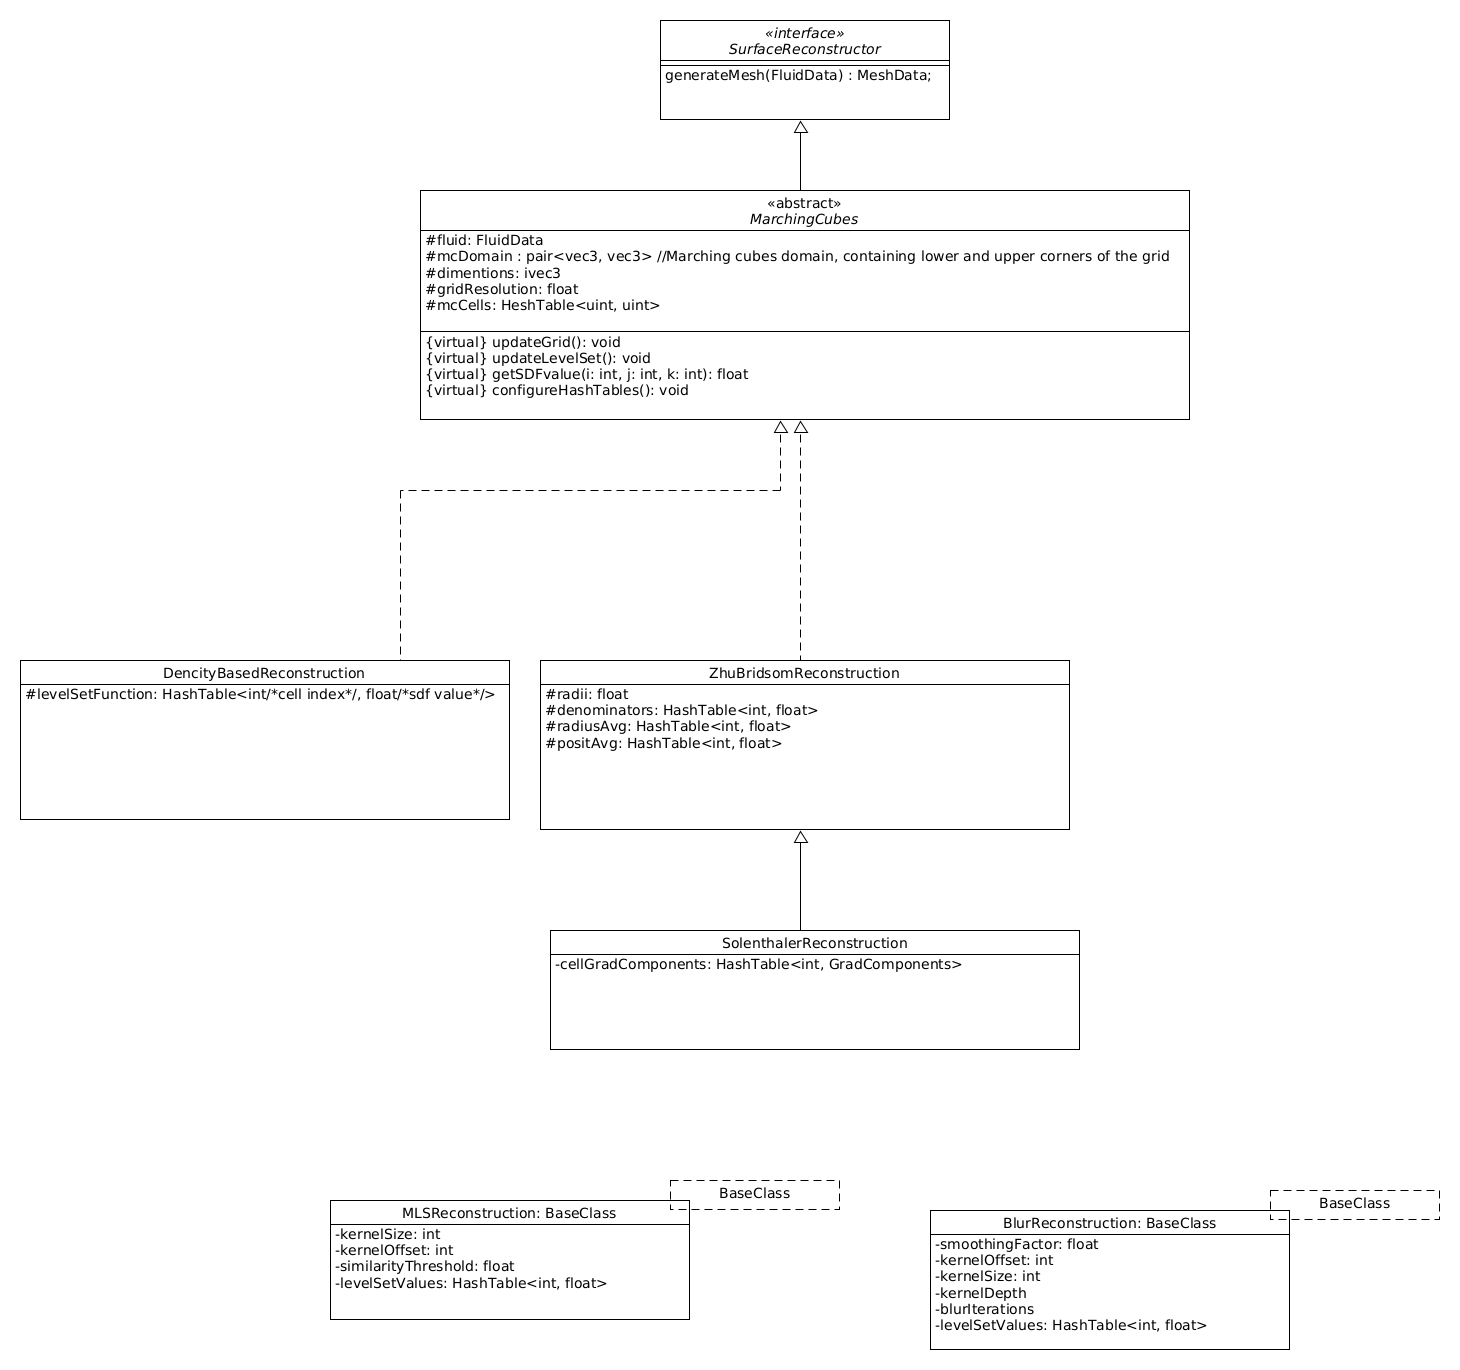
\includegraphics[width=150mm]{figures/ClassDiagram.pdf}
	\end{center}
	\caption{Class diagram, representing inheritance architecture for the surface reconstruction methods}
    \label{fig:class-diagam}
\end{figure}
The base class for all reconstruction methods is \emph{MarchingCubes} class. This class contains common properties for all methods, which exploits Marching Cubes algorithm. Here \emph{mcDomain} is a pair of two points, representing the domain of marching cubes in 3d space, \emph{dimensions} - is a vector, containing number of MC grid cells in X, Y and Z directions, \emph{gridResolution} - the size of each cell (all cells are assumed to be of a uniform size where $width=length=height$), \emph{mcCells} - is a hash table which contains key-value pairs of cell index and number of SPH fluid particles within its support radius. Each MC cell vertex has its unique integer index, which can be transformed from its position in 3d space. The transformations are extensively explained in \cite{Akinchi}. 
The \emph{MarchingCubes} class has 4 virtual methods, which should be reimplemented inside each subclass:
\begin{itemize}
	\item \emph{configureHashTables()} - inside this method every concrete method performs initial configuration of hash tables, which are used to compute SDF.
	\item \emph{updateGrid()} - computes the cells domain where calculation of SDF will be performed.
	\item \emph{updateLevelSet()} - updates hash tables with data, required to compute level set values
	\item \emph{getSDFvalue} - calculates resulting SDF value for a given MC cell vertex
\end{itemize}

\emph{MarchingCubes} class re-implements interface method \emph{generateMesh()} composing previously defined functions (see Algorithm \ref{alg:generateMesh}).

\begin{algorithm}
	\caption{General overview of the algorithm applied inside each concretisation of MarchingCubes class}
	\label{alg:generateMesh}
	\begin{algorithmic}
		\State $configureHashTables()$
		\State $updateGrid()$
		\State $updateLevelSet()$
		\State $mesh \gets computeMesh()$ 
		\State $return mesh$
	\end{algorithmic}
\end{algorithm}

\section{Adaptive hash tables for Marching Cubes grid}
As described in \cite{Akinchi} the computation time for extracting smooth surfaces is mainly influenced by
the resolution of the Marching Cubes grid and the smoothing radius R and achieving high quality surfaces is possible at the expense of performance. One of the main causes of this issue is computing the scalar field over the volume of the fluid instead of concentrating on the surface area. Thus for performance and memory optimization reasons we decided to apply suggestions, proposed in \cite{Akinchi}.

First step is to determine MC grid domain, on which all computation operations will be performed. To perform fluid surface reconstruction it is enough to compute SDF for a MC grid cells that are near the fluid surface. To determine compute \emph{surface cells vertices} we have to:
\begin{itemize}
		\item Compute fluid particles, that are in the near neighborhood to the surface of the fluid. In order to determine surface particles in a preprocessing step, the smoothed color field method \cite{ColorField} is employed.  The smoothed color field value of a particle at position x is computed using Equation \ref{eq:ColorField}.
		\item For each determined particle compute MC grid vertices, that are within the support radius R from each SPH particle, computed in previous step 
\end{itemize}
\begin{equation} \label{eq:ColorField}
	cf_i = \sum_{j\in SPHNeighbors_i}{m_j \cdot \dfrac{W_{ij}}{\rho_j}}
\end{equation}
Where:
\begin{conditions}
	SPHNeighbors_i & set of neighbor fluid particles for particle i\\
	W_{ij} & kernel function\\
	\rho_j & density of particle j\\
\end{conditions}
Detailed instructions sequence described in Algorithm \ref{alg:MC_grid_domain_computation}.
\begin{algorithm}
	\caption{Compute MC grid vertices near the SPH surface}
	\label{alg:MC_grid_domain_computation}
	\begin{algorithmic}
		\ForAll{ $i \in ParticleSet$}
			\State Compute CF using Equation \ref{eq:ColorField}
			\If{$CF \in ThresholdRange$}
				\State $ParticleSet \gets ParticleSet - i$
			\EndIf

		\EndFor
		\ForAll{$i \in ParticleSet$}
			\State Compute $Neighbors_i$ of MC vertices within R from  i
			\State $MCGridDomain \gets MCGridDomain \cup Neighbors_i$
		\EndFor
		\State return MCGridDomain
	\end{algorithmic}
\end{algorithm} 

\section{Results}

The results of the reconstruction using previously described methods on Figure \ref{fig:rec_methods}.
\begin{figure}[H]
	\begin{subfigure}[b]{\textwidth}
		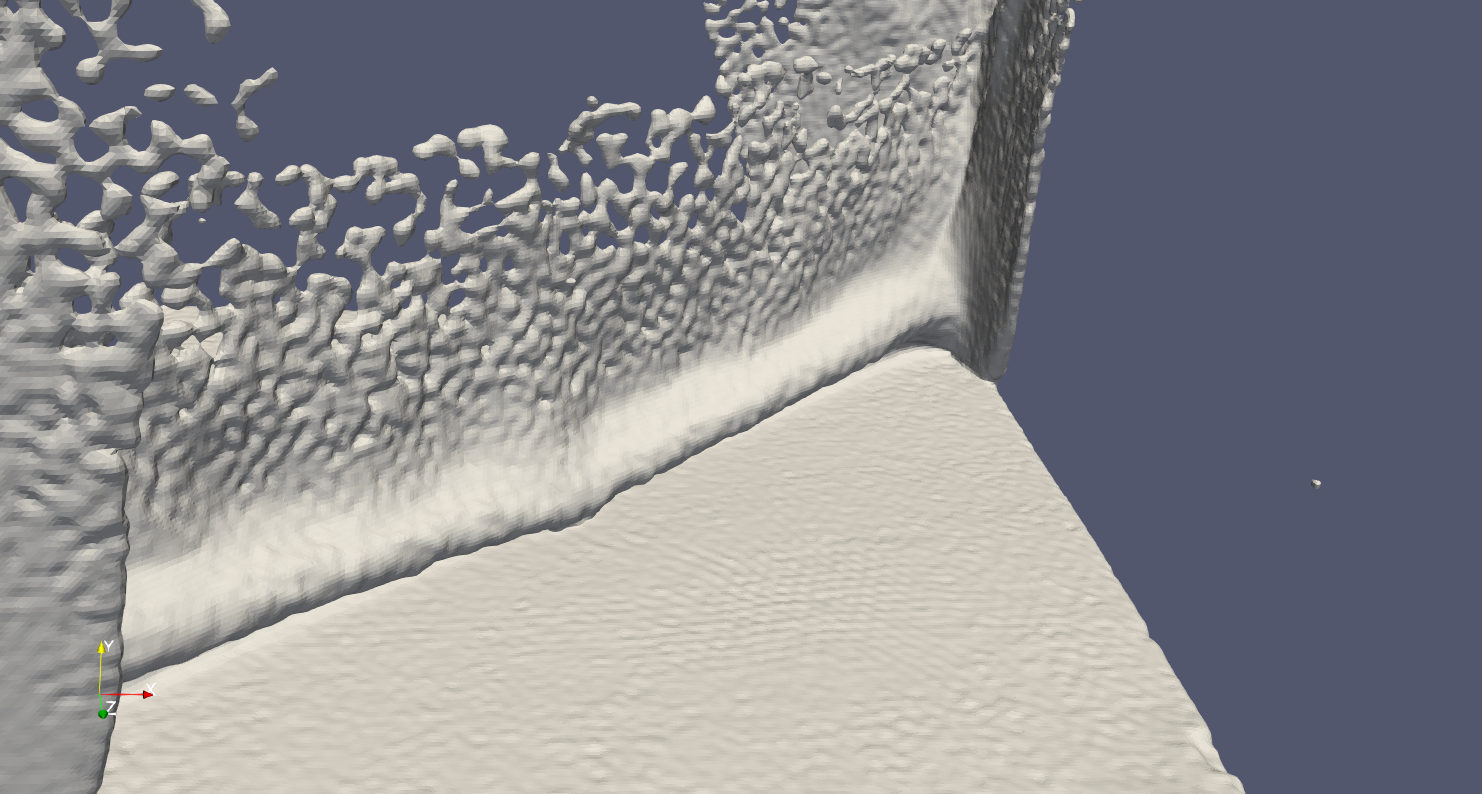
\includegraphics[width=\textwidth]{figures/DencityBasedReconstruction.png}
		\caption{Density-based reconstruction \cite{DencRec}}
	\end{subfigure}
	\begin{subfigure}[b]{\textwidth}
		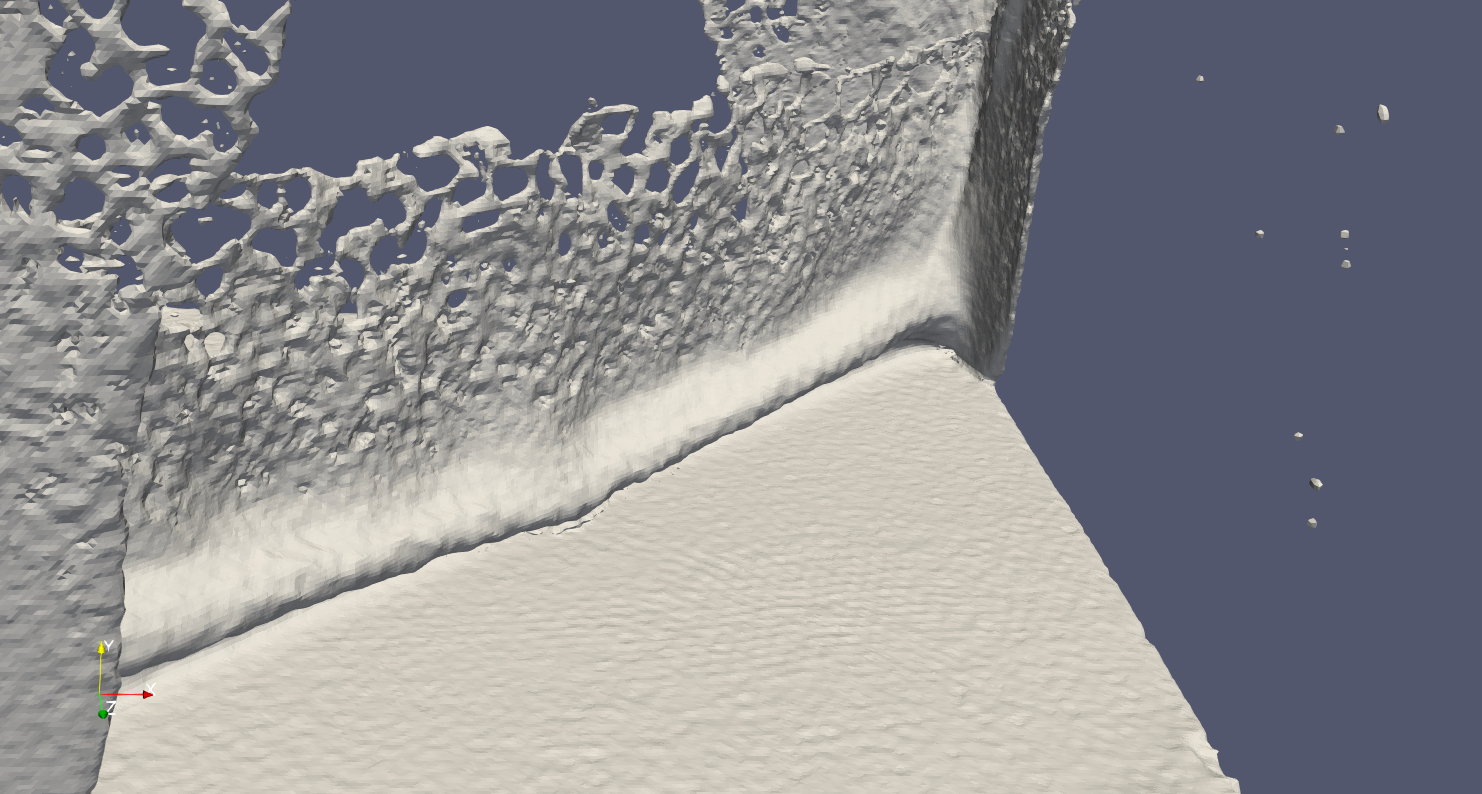
\includegraphics[width=\textwidth]{figures/ZhuBridsonReconstruction.png}
		\caption{Zhu and Bridson reconstruction \cite{ZhuBridson}}

	\end{subfigure}
	\begin{subfigure}[b]{\textwidth}
		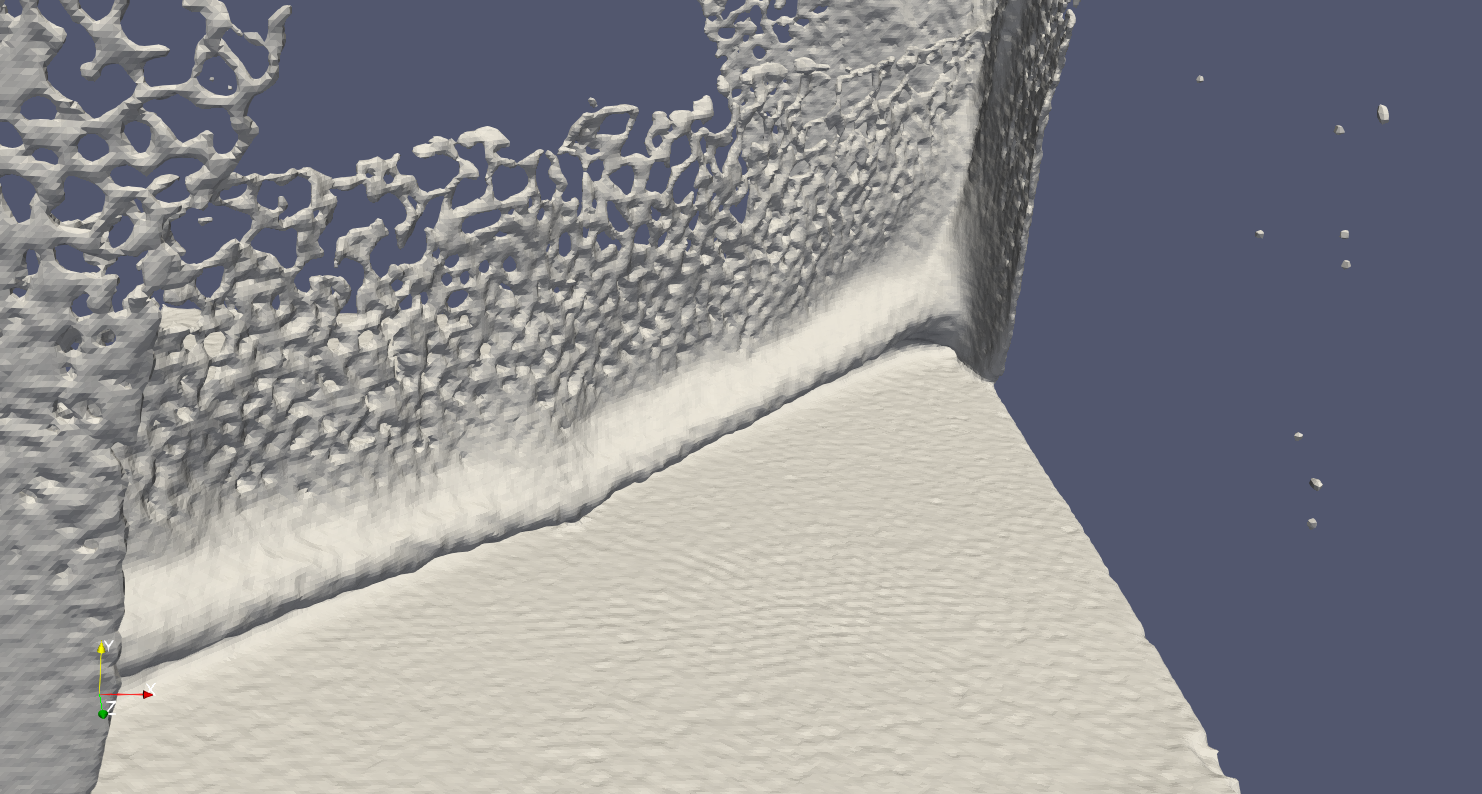
\includegraphics[width=\textwidth]{figures/SolenthilerReconstruction.png}
		\caption{Solenthaler reconstruction \cite{Solenthaler}}

	\end{subfigure}
	\label{fig:rec_methods}
\end{figure}
Each method has different quality of the reconstructed surface due to the SDF computation approach. In this case Zhu-Bridson and Solenthaler methods at it fundamental have a similar approach of computing SDF, but Additional to this Solenthaler method removes artifacts in concave regions, that are inherent for Zhu-Bridson reconstruction method.

